\input{../phil140b.tex}
\usepackage{amsmath, dsfont, mathtools, verbatim, tikz, float}

\usetikzlibrary{arrows,automata}

\oddsidemargin 0in
\evensidemargin 0in
\textwidth 6.5in
\topmargin -0.5in
\textheight 9.0in
\newcommand{\norm}[1]{\left\lVert #1 \right\rVert}
\newcommand{\?}{\stackrel{?}{=}}
\DeclarePairedDelimiter{\ceil}{\lceil}{\rceil}

\begin{document}

\solution{Nikhil Unni}{Assignment \#1}{Spring 2016}
\pagestyle{myheadings}

\begin{enumerate}
  \item
    {\it 
    Assume as given the fundamental theorem of algebra to the effect that every polynomial equation of degree $n$ has exactly $n$ roots (not necessarily distinct) over the complex numbers. Show that the set of roots in the complex numbers which are solutions of cubic equations of the form $x^3 + ax^2 + bx + c = 0$ ($a, b, c$ are positive natural numbers) is an enumerable set.\\
    }

    Before we can solve the problem there's a preliminary proof : we need to show that the Cartesian product of two enumerable sets is enumerable. Say we have two enumerable sets, $S$ and $T$. For simplicity, let's assume that the two sets are countably infinite, and thus have a bijection with $\mathds{N}^+$. Without loss of generalization, say that the sets are enumerated like $S = \{s_1, s_2, \dots\}$ and $T = \{t_1, t_2, \dots \}$. Inspired by Cantor's diagonal argument, we can order $S \times T$ like:

    \begin{tabular}{ l l l l }
      $(s_1, t_1)$ & $(s_1, t_2)$ & $(s_1, t_3)$ & $\dots$ \\
      $(s_2, t_1)$ & $(s_2, t_2)$ & $(s_2, t_3)$ & $\dots$ \\
      $(s_3, t_1)$ & $(s_3, t_2)$ & $\ddots$ \\
    \end{tabular}

    And we can enumerate this set by taking elements ``peeling outward'' from $(s_1,t_1)$. Each ``layer'' after $(s_1,t_1)$ is finitely long -- namely -- there are $2n - 1$ elements in the $n$th layer. The first layer is $\{ (s_1, t_1) \}$, the second layer is $\{ (s_1, t_2) , (s_2, t_2), (s_2, t_1) \}$, etc, etc. Through this scheme, we'll enumerate every element of $S \times T$, and thus the Cartesian product is enumerable as well.\\

    Now, we can first show that the set of all cubic equations of the given form is an enumerable set. There's a clear bijection between the set of all cubic equations of the form $x^3 + ax^2 + bx + c = 0$ with $a,b,c \in \mathds{N}^+$ and $\mathds{N}^+ \times \mathds{N}^+ \times \mathds{N}^+$ : $(a,b,c) \mapsto x^3 + ax^2 + bx + c = 0$. Since $\mathds{N}^+$ is enumerable, $\mathds{N}^+ \times \mathds{N}^+$ is enumerable, and so $\mathds{N}^+ \times (\mathds{N}^+ \times \mathds{N}^+)$ is enumerable. And there's a clear bijection between $\mathds{N}^+ \times (\mathds{N}^+ \times \mathds{N}^+)$ and $\mathds{N}^+ \times \mathds{N}^+ \times \mathds{N}^+$ : $(x, (y,z)) \mapsto (x,y,z)$.\\

     As noted in the problem statement, for each equation of the form $x^3 + ax^2 + bx + c = 0, a,b,c \in \mathds{N}^+$ (call this set $\mathds{P}$), there are exactly 3 complex roots. Since we can enumerate the polynomials, there's a bijection with the positive natural numbers. Call this $f : \mathds{N}^+ \rightarrow \mathds{P}$. We can define another bijection between $\mathds{N}^+$ and the set of all complex roots of $\mathds{P}$ (call this $\mathds{D}$). We can define a bijection $g : \mathds{N}^+ \rightarrow \mathds{D}$. Given some positive natural number, $n$, we can find the corresponding polynomial : $f( \ceil{n/3} )$, and of the 3 complex roots, we pick the $(n \mod 3)$th root. We can arbitrarily order complex numbers $a + bi$ by ordering by $a$ first, then $b$. This way, we can deterministically pick a complex root, and all possible roots can be picked with this scheme, meaning we have a valid bijection.\\

     To put it simply, if we have the polynomials ordered like $p_1, p_2, p_3, \dots$ we can order the roots like $r_{1,1}, r_{1,2}, r_{1,3}, r_{2,1} \dots$. And thus, the set of all possible complex roots is enumerable.\\

  \item 
    {\it 
      Show that the set of partial functions $f : \mathds{N}^+ \rightarrow \{1,2,3,4\}$ cannot be enumerated. (With $\mathds{N}^+ = \{1,2,3,\dots\}$)\\
    }

    The cardinality of the set of partial functions from $\mathds{N}^+$ to $\{1,2,3,4\}$ is strictly greater than the cardinatlity of the set of all subsets of $\mathds{N}^+$, since a partial function is a map from a subset of the domain to a subset of the codomain. So if the powerset is $\mathds{N}^+$ is not enumerable, then the set of all partial functions must not be enumerable as well.\\

    Assume that the powerset of $\mathds{N}^+$ is enumerable. Then, there exists a bijection $f: \mathds{N^+} \rightarrow 2^{\mathds{N}^+}$. Let's construct a set of natural numbers:
    $$S = \{x \in \mathds{N}^+ : x \not \in f(x) \}$$
    Because $S$ is some set of natural numbers, we know $S \in 2^{\mathds{N}^+}$. And because we have our bijection, there exists some $n \in \mathds{N}^+$ such that $n = f^{-1}(S)$. If $n \in S$, then $n \not \in f(n)=S$ by the definition of $S$ -- which is a contradiction. Conversely if $n \not \in f(n)=S$, by the definition of $S$, $n$ should be included in $S$ -- again, leading to a contradiction. Because we have a contradiction both ways, there cannot exist such a bijection, and thus we know that $2^{\mathds{N}^+}$ cannot be enumerable. It then follows that the set of all partial functions from $\mathds{N}^+$ to $\{1,2,3,4\}$ must not be enumerable as well.
    
  \item 
    {\it
      Consider a tape containing a block of $n$ strokes, followed by a space, followed by a block of $m$ strokes, followed by a space, followed by a block of $k$ strokes, and otherwise blank. Design a Turing machine that when started on the leftmost stroke will eventually halt, having neither printed nor erased anything...
    }
    \begin{itemize}
      \item [a] {\it ... on the leftmost stroke of the second block.}\\

        \begin{figure}[H]
        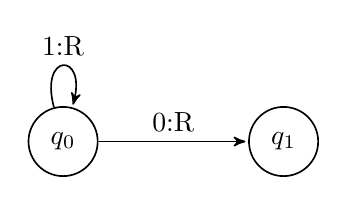
\begin{tikzpicture}[->,>=stealth',shorten >=1pt,auto,node distance=2.8cm, semithick]
          \tikzstyle{every state}=[fill=none,draw=black,text=black]
          \node[state] (A)              {$q_0$};
          \node[state] (B) [right of=A] {$q_1$};

          \path (A) edge              node {0:R}   (B)
                    edge [loop above] node {1:R}   (A);
        \end{tikzpicture}
        \end{figure}

        We skip over the entire first block until we hit a 0, and then move over by 1, which will land on the leftmost of the second block.

      \item [b] {\it ... on the leftmost stroke of the third block.}\\

        \begin{figure}[H]
        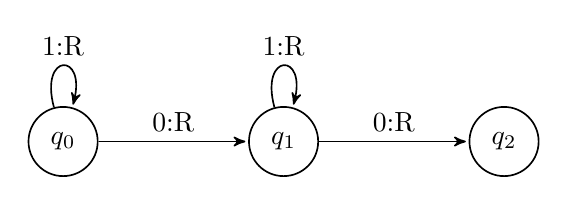
\begin{tikzpicture}[->,>=stealth',shorten >=1pt,auto,node distance=2.8cm, semithick]
          \tikzstyle{every state}=[fill=none,draw=black,text=black]
          \node[state] (A)              {$q_0$};
          \node[state] (B) [right of=A] {$q_1$};
          \node[state] (C) [right of=B] {$q_2$};

          \path (A) edge              node {0:R}   (B)
                    edge [loop above] node {1:R}   (A)
                (B) edge              node {0:R}   (C)
                    edge [loop above] node {1:R}   (B);
        \end{tikzpicture}
        \end{figure}

        Now we do the same as the machine above, but we have to go over two blocks of 1, with two 0 transitions denoting the spaces between block 1/block 2 and block 2/block 3.

    \end{itemize}
  \item 
    {\it
      Design a Turing Machine to compute the function max(x,y) = the larger of x and y.
    }

    Actual Turing Machine figured on the next page. \\

    For each stroke in x, we try to find a corresponding rightmost stroke in y, and move the leftmost stroke in x by 1 over, and moving the rightmost stroke in y by 1 over. Then, we recenter back to the original starting point (now looking at x-1 and y-1). This continues until either x or y is 0, in which case we wipe out the other strokes, and combine the max of the two. Recall that after moving over, now the max(x,y) is split up into two pieces, separated by one empty stroke, so then it's a simple addition operation of the ``winner'' of x and y.

    \begin{figure}[!htbp]
      \caption{Turing Machine for max(x,y)}
      \centering
      \includegraphics[width=1.1\textwidth]{states}
    \end{figure}
    
\end{enumerate}

\end{document}
